
\section{Hadronic Calorimeter}

The Hadronic Calorimeter (HCAL) is devoted to absorb and measure the energy of final states hadrons. Together with the ECAL, it plays a key role on the jet reconstruction and missing energy measurement. It is the last subdetector until the magnet coil and, as much as possible, tries to cover the largest pseudorapidity region in order to enhance the missing transverse energy identification. It is composed by layers of brass and steel, interleaved with plastic scintillators, with 3.7 mm thickness each, in order to leave as much as possible space for the absorptive materials. This alows, once a hadron hit the material, the formation of hadronic cascades. These cascades are detected by the scintillators which emits light proportional to the amount of energy deposited.

The HCAL is divided in 4 components, the HB (barrel) 9 m long in the central region

In the region $\abs{\eta} < 1.74$, the HCAL cells have widths of 0.087 in pseudorapidity and 0.087 in azimuth ($\phi$), corresponding to 5 to 10 interaction lengths. In the $\eta$-$\phi$ plane, and for $\abs{\eta} < 1.48$, the HCAL cells map on to $5 \times 5$ arrays of ECAL crystals to form calorimeter towers projecting radially outwards from close to the nominal interaction point. For $\abs{\eta} > 1.74$, the coverage of the towers increases progressively to a maximum of 0.174 in $\Delta \eta$ and $\Delta \phi$. Within each tower, the energy deposits in ECAL and HCAL cells are summed to define the calorimeter tower energies, which are subsequently used to provide the energies and directions of hadronic jets. Figure~\ref{cms_hcal} shows a longitudinal view of the HCAL.

% cms hcal
\begin{figure}[htbp]
    \centering
    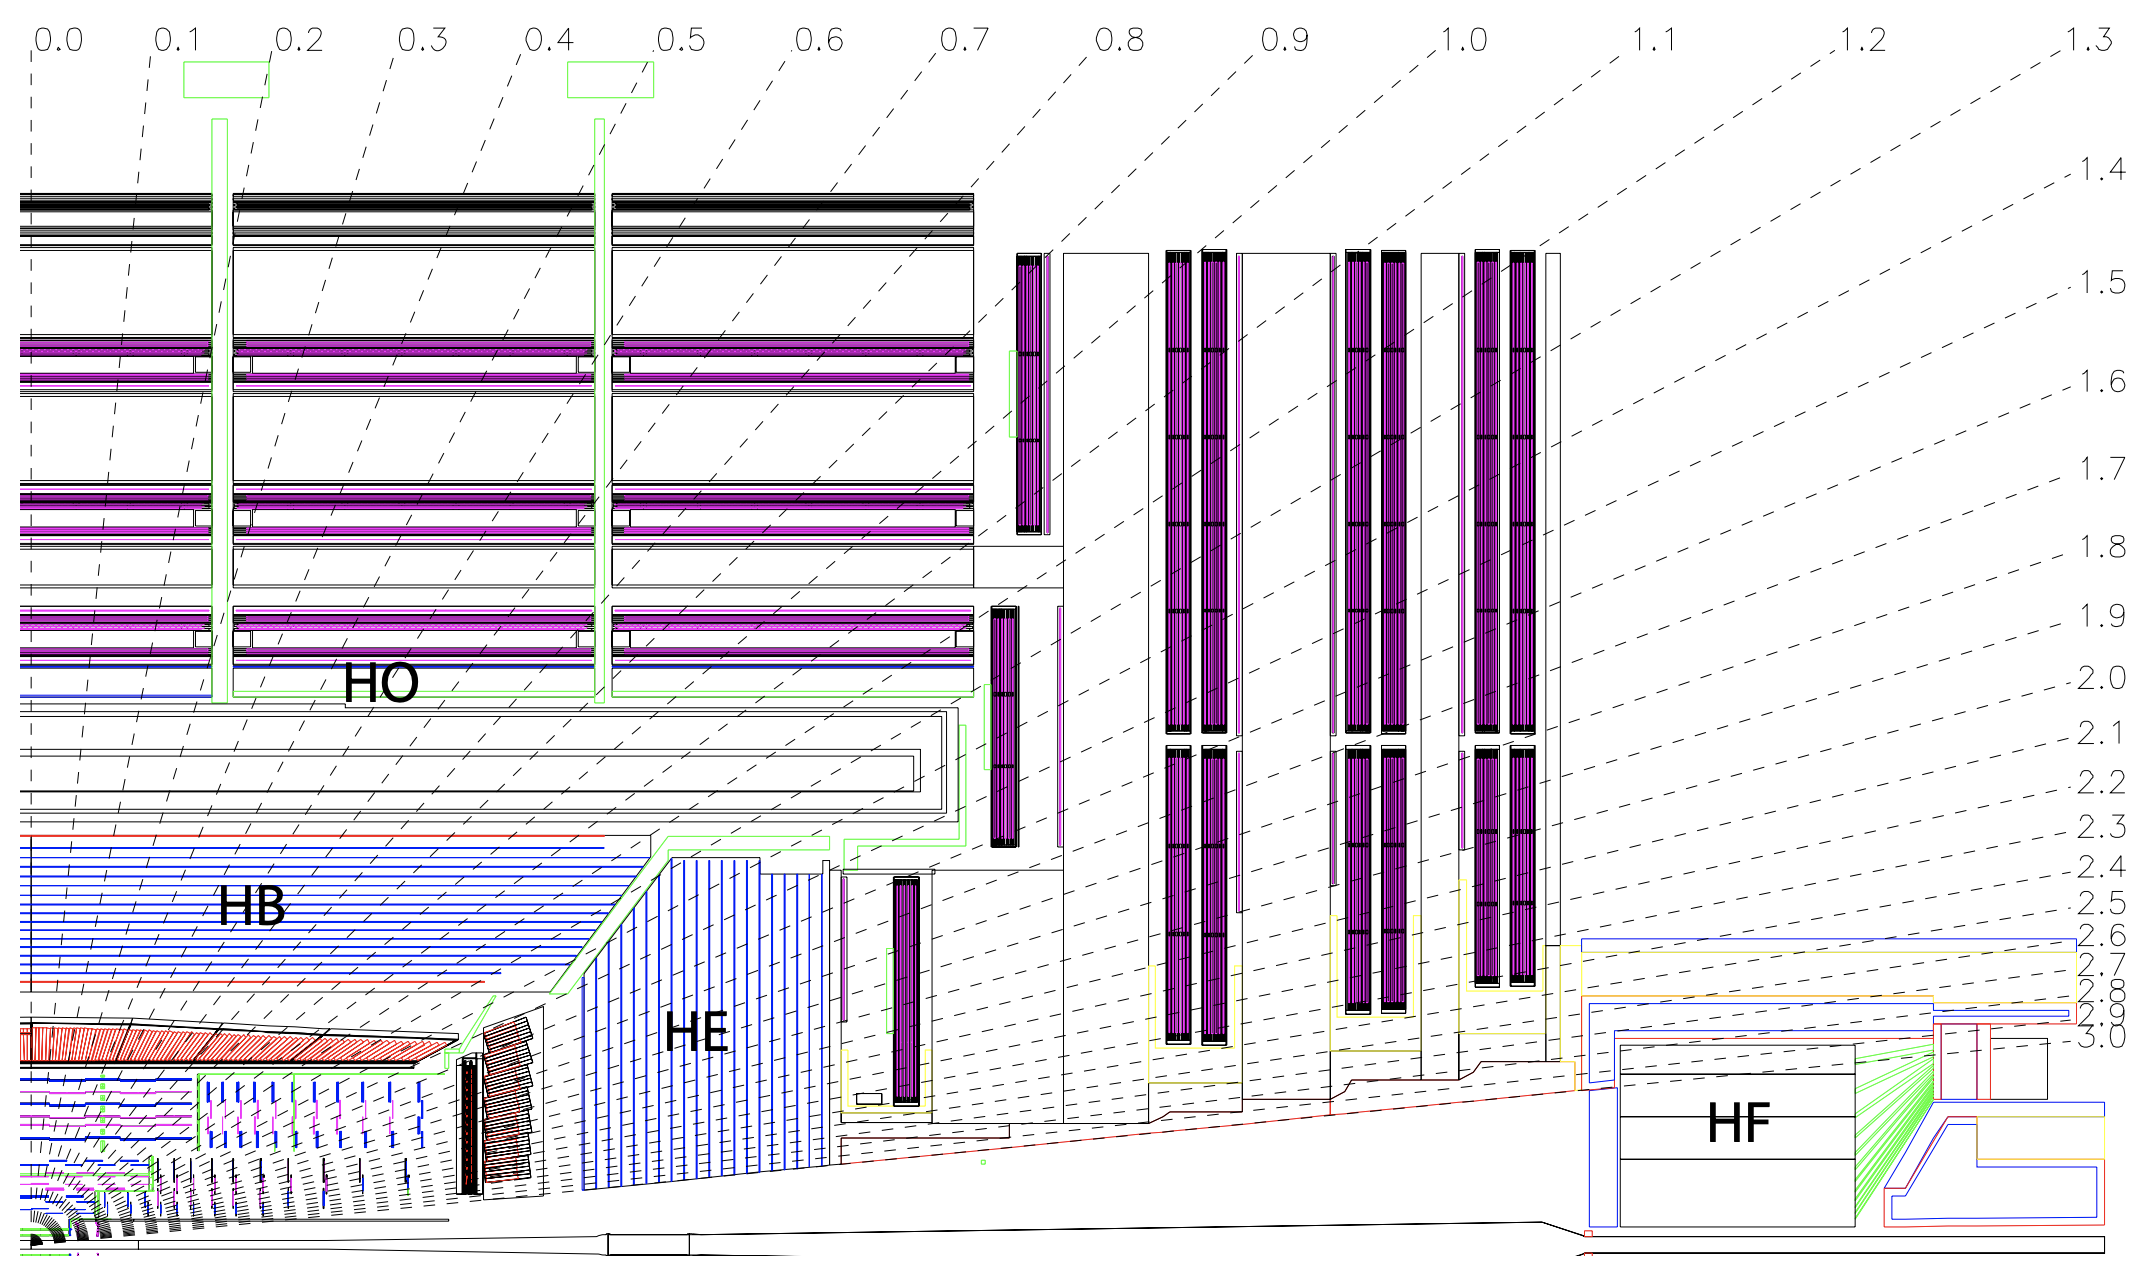
\includegraphics[width=0.9\textwidth]{figures_and_tables/experimental_setup/cms_hcal.png}
    \caption{Longitudinal section view of the HCAL and its components. The barrel calorimeter (HB) covers the central region, inside the solenoid, the outer calorimeter covers also the central region, but it is positioned on the outside the solenoid. The endcap calorimeter (HE) covers the forward region and it is complemented by the forward calorimeter (HF), which uses Cherenkov light detectors made of radiation-hard quartz fibers. Source:~\cite{Chatrchyan:2008zzk}.}
    \label{cms_hcal}
\end{figure}

Jets are reconstructed offline from the energy deposits in the calorimeter towers, clustered using the anti-\kt algorithm~\cite{Cacciari:2008gp, Cacciari:2011ma} with a distance parameter of 0.4. In this process, the contribution from each calorimeter tower is assigned a momentum, the absolute value and the direction of which are given by the energy measured in the tower, and the coordinates of the tower. The raw jet energy is obtained from the sum of the tower energies, and the raw jet momentum by the vectorial sum of the tower momenta, which results in a nonzero jet mass. The raw jet energies are then corrected to establish a relative uniform response of the calorimeter in $\eta$ and a calibrated absolute response in transverse momentum \pt.

